%% LaTeX2e class for student theses
%% sections/content.tex
%% 
%% Karlsruhe Institute of Technology
%% Institute of Information Security and Dependability (KASTEL)
%%
%% Template by
%% Dr.-Ing. Erik Burger
%% burger@kit.edu
%%
%% Adaption by
%% Annika Vielsack
%% vielsack@kit.edu
%%
%% Version 1.0, 2021-07-03
\definecolor{codegreen}{rgb}{0,0.6,0}
\definecolor{codegray}{rgb}{0.5,0.5,0.5}
\definecolor{codepurple}{rgb}{0.58,0,0.82}
\definecolor{backcolour}{rgb}{0.95,0.95,0.92}

\lstdefinestyle{mystyle}{
    backgroundcolor=\color{backcolour},   
    commentstyle=\color{codegreen},
    keywordstyle=\color{magenta},
    numberstyle=\tiny\color{codegray},
    stringstyle=\color{codepurple},
    basicstyle=\ttfamily\footnotesize,
    breakatwhitespace=false,         
    breaklines=true,                 
    captionpos=b,                    
    keepspaces=true,                 
    numbers=left,                    
    numbersep=5pt,                  
    showspaces=false,                
    showstringspaces=false,
    showtabs=false,                  
    tabsize=2
}

\lstset{style=mystyle}
\chapter{Preliminary Knowledge}
\label{ch:Backgroud}

\section{History}
\label{sec:Backgroud:History}


\section{Bitcoin}
\label{sec:Backgroud:Bitcoin}

\section{Ethereum}
\label{sec:Backgroud:Ethereum}

\section{Smart Contract}
\label{sec:Backgroud:SmartContracts}


\section{Security Analysis}
\label{sec:Backgroud:SecurityAnalysis}



\chapter{Most Common Vulnerabilities}
\label{ch:Vulnerabilities}

Presentation of what effected the smart contrats in the recent year.
The vulnerabilities that I found more often in papers that I read and I selected because I think they are the 
most rappresentative and the most common used by the attackers.

As introduction, I cite some papers that I read dealing with this topic. I select the following vulnerabilities, because I think they represent a risk still today.

\section{Race Codition}
\label{sec:Vulnerabilities:RaceCondition}
Race condition represents in computer science one of the most common vulnerabilities.
\citet{RaceConditionDef} identifies this as an even,  which occurs when two threads access a shared variable at the same time.
A case is illustruted when two threads read the value of a shared variable. After computing operations on that, they update the shared variable. The change applied by the last thread will be preserved and the other one will be lost.
In a Solidity context an analogous situation can happen. This can be exploited by attackers, for withrowing a higher amount of token or manipulating the price of it.
\autoref{lst:EchidnaCode}
\citetitle{NotSoSmartContracts} is a repository that contains examples of common Ethereum smart contract vulnerabilities.
Vulnerable smart contracts and explanations are coupled and presented. I considered the smart contract \href{https://github.com/crytic/not-so-smart-contracts/blob/master/race_condition/RaceCondition.sol}{RaceCodition.sol} for showing a case of this class of vulnerability.
The vulnerability relies on the shared variable price, which is updated by the function changePrice (\autoref{lst:RaceCodition} line 15) and used by the function buy (\autoref{lst:RaceCodition} line 2).
\begin{lstlisting} [language={Solidity},caption={Cross-function RaceCondition vulnerable functions.}, label={lst:RaceCodition}]

    function buy(uint new_price) payable
        public
    {
        require(msg.value >= price);

        // we assume that the RaceCondition contract
        // has enough allowance
        token.transferFrom(msg.sender, owner, price);

        price = new_price;
        owner = msg.sender;
    }

    function changePrice(uint new_price){
        require(msg.sender == owner);
        price = new_price; 
    }    
\end{lstlisting}

When a user tries to buy tokens, the owner can call the function for changing the price of the token, consequently the attacked user will spend more than he expected.
 

\section{Denial Of Services}

The article \citet{CloudFareDos} of CloudFare, proposes a definition of denial-of-service (DoS) attack. It is a type of cyber attack in 
which an attacker aims to render a computer or a informatic service (logical or phisical) unavailable to its intended users by interrupting the 
device's normal functioning. 

In Solidity contetext, DoS consists of attacks where 
users can leave the contract inoperable for a small period of time, or in some cases, permanently.
It represents a cathegory of attacks, consequently it is not possible to classify a 
spefic vulnerability or methodology for exploiting a thread.

As an example of this class of attack, I selected the smart contract presented by \citet{Dos1}. 
It allows the user to place a bid to the contract. If it is the highest bid, it 
sends the previous leader the current bid and set the leader to the sender with the new highest bid.
The vulnerability relies on line 12 (\refname{lst:DosContract1}): the require condition is respected if the transaction which refunds the old leader doesn not revert. 
An attacker can exploit this vulnerability, creating a smart contract which cannot receive ether. Then it intacts with the vulnerable contract, becoming the leader.
When the vulnerable tries to refund the attacker one, it will always revert because it cannot receive ether and no one could become the new leader.

\begin{lstlisting} [language={Solidity},caption={Dos Vulnerable Contract.}, label={lst:DosContract1}]
    pragma solidity ^0.8.0;

    /**
     * @title VulnerableContract
     * @dev This contract is vulnerable to a denial of service (DoS) attack
     */
    contract VulnerableContract {
        address payable leader;
        uint256 public highestBid;
    
        function bid() external payable {
            require(msg.value > highestBid);
    
            // Refund the old leader, if it fails then revert
            require(leader.send(highestBid));
    
            leader = payable(msg.sender);
            highestBid = msg.value;
        }
    
        /// Helper function to check leader
        function getLeader() external view returns (address) {
            return leader;
        }
    }
    
\end{lstlisting}

\chapter{Real world Exploits}
\label{ch:Exploits}
Real-wolrd exploits that have happend in the recent years.

The structure of this chapter is 
\begin{itemize}
    \item explanation of the protocol
    \item the exploit 
    \item the properties involved, which will be analysed by the tools
\end{itemize}

Brief explanation of the terminology used -> postcondition precondtion invariant


\section{\$34 Million stacks NFT Project Aku Dreams Smart Contract}
\label{sec:Exploits:AkuDreams}
\href{https://www.business2community.com/nft-news/nft-market-size-how-to-track-02467120}{Business2community} estimates the value of NFT market around \$100 billion.
Nowadays, the word NFT is one of the most researched ones on Google and the other search engine.
NFT's marketplaces manage the transaction behind these valuable markets. 
They are made by a frontend part, but even by a backend one which relies on the blockchain. 
Akutars, a highly anticipated Ethereum-based NFT project developed by Aku Dreams, is an example of how a bug can have catastrophic consequences in this sector. 

\subsection{Akutarts NFT project}
\label{sec:AkuDreams:Akutars}
\cite{Aku} reports Akutarts locked up \$34 million due to the faulty code of the smart contract.
The launch contained 15,000  NFTs and was based on the Dutch auction. This strategy involves a descending price auction where an item begins at a set maximum price. 
The price is gradually lowered over a fixed time until a bid is placed that guarantees the bidder the purchase of the item at the current price. 
Anyone who paid the higher amount would get a refund.
Unfortunately, the launch was corrupted, since the errors in the codes made the project open to exploits. 
An attacker could block the withdrawals and refunds while attempting to highlight the vulnerabilities within the project.

\subsection{The exploit}
\label{sec:AkuDreams:AkutarsExploit}

The first part of the exploit involved the function processRefunds \autoref{lst:AkuDreamsProcessRefunds}.

This has the aim to refund the bid of the user who took part in the auction. 

The problem relies on the for loop in line 11. 
It loops on all over the users, who needs to be refunded, estimating the number of tokens to send. 
Then, the amount is sent with the function call, which returns a boolean, based on the correct execution of the operation.
This is checked with a require, line 22; so, if the operation concluded incorrectly, it would revert the transaction.

The problem relies on the require in the loop. If one of the accounts could not receive the refund, the function would always reverted.
Since looping all over the users is a sequential operation, if the transaction just reverted when it reaches an item, it would never reach all the following items. 

Therefore, a malicious user just implemented a smart contract which took part in the auction and reverted any time it received tokens.

\begin{lstlisting} [language={Solidity},caption={Function for refunding the users.}, label={lst:AkuDreamsProcessRefunds}]
    function processRefunds() external {
      require(block.timestamp > expiresAt, "Auction still in progress");
      uint256 _refundProgress = refundProgress;
      uint256 _bidIndex = bidIndex;
      require(_refundProgress < _bidIndex, "Refunds already processed");
      
      uint256 gasUsed;
      uint256 gasLeft = gasleft();
      uint256 price = getPrice();
      
      for (uint256 i=_refundProgress; gasUsed < 5000000 && i < _bidIndex; i++) {
          bids memory bidData = allBids[i];
          if (bidData.finalProcess == 0) {
            uint256 refund = (bidData.price - price) * bidData.bidsPlaced;
            uint256 passes = mintPassOwner[bidData.bidder];
            if (passes > 0) {
                refund += mintPassDiscount * (bidData.bidsPlaced < passes ? bidData.bidsPlaced : passes);
            }
            allBids[i].finalProcess = 1;
            if (refund > 0) {
                (bool sent, ) = bidData.bidder.call{value: refund}("");
                require(sent, "Failed to refund bidder");
            }
          }
          
          gasUsed += gasLeft - gasleft();
          gasLeft = gasleft();
          _refundProgress++;
      }

      refundProgress = _refundProgress;
    }
\end{lstlisting}
The second part of the exploit is characterized by a bug in the logic, which could not allow the developer team to withdraw the project funds. 

The function claimProjectFunds (\autoref{lst:AkuDreamsClaim}), callable only by the owner of the contract due to the modifier onlyOwner, 
refunds the developers just when all the users are considered refunded. 

The boolean condition, contained in the require at line 3, is the heart of the problem. 
The require compares the variable refundProgress, which takes track of the refund progress, 
and totalBids.
\begin{lstlisting} [language={Solidity},caption={Function for claiming the funds for the developers.}, label={lst:AkuDreamsClaim}]
    function claimProjectFunds() external onlyOwner {
        require(block.timestamp > expiresAt, "Auction still in progress");
        require(refundProgress >= totalBids, "Refunds not yet processed");
        require(akuNFTs.airdropProgress() >= totalBids, "Airdrop not complete");

        (bool sent, ) = project.call{value: address(this).balance}("");
        require(sent, "Failed to withdraw");        
    }
\end{lstlisting}

The variable totalBids is increased every time a bid is placed, regardless of the user who computed it, shown in \autoref{lst:AkuDreamsBid} at line 18.
The user can call the function \_bid, for placing a bid, with an arbitrary amount of bids, but the variable refundProgress is increased every time a user is refunded. 
Consequently, if a user bought more than one bid, the amount of refounded users would never be greater or equal to the number of placed bids.
\begin{lstlisting} [language={Solidity},caption={Function for users'bid}, label={lst:AkuDreamsBid}]
    function _bid(uint8 amount, uint256 value) internal {
        require(block.timestamp > startAt, "Auction not started yet");
        require(block.timestamp < expiresAt, "Auction expired");
        uint80 price = getPrice();
        uint256 totalPrice = price * amount;
        if (value < totalPrice) {
            revert("Bid not high enough");
        }
        
        uint256 myBidIndex = personalBids[msg.sender];
        bids memory myBids;
        uint256 refund;

        if (myBidIndex > 0) {
            myBids = allBids[myBidIndex];
            refund = myBids.bidsPlaced * (myBids.price - price);
        }
        uint256 _totalBids = totalBids + amount;
        myBids.bidsPlaced += amount;

        if (myBids.bidsPlaced > maxBids) {
            revert("Bidding limits exceeded");
        }

        if(_totalBids > totalForAuction) {
            revert("Auction Full");
        } else if (_totalBids == totalForAuction) {
            expiresAt = block.timestamp; //Auction filled
        }

        myBids.price = price;

        if (myBidIndex > 0) {
            allBids[myBidIndex] = myBids;
        } else {
            myBids.bidder = msg.sender;
            personalBids[msg.sender] = bidIndex;
            allBids[bidIndex] = myBids;
            bidIndex++;
        }
        
        totalBids = _totalBids;
        totalBidValue += totalPrice;

        refund += value - totalPrice;
        if (refund > 0) {
            (bool sent, ) = msg.sender.call{value: refund}("");
            require(sent, "Failed to refund bidder");
        }
    }
\end{lstlisting}

\subsection{Properties}
The smart contract involves 2 main problems: the refunding of the users who placed the bids and the claim of the developers' rewards.

The first property deals with the function processRefunds. 
It reverts every time because a malicious wallet, which can't receive 
any tokens triggering the require. 
We verify if the contract can always refund all the users.
The property involves the sum of refunded wallets may be equal to the number of the counter which loops on the map containing the data. 
It is a postcondition, so it is proven that all the users are refounded if the function does not revert, which means that the function does not 
consider the case of error.

The other property regards the function claimProjectFunds. 
In the beginning, some requirements have to be fulfilled before the owner can obtain the rewards.
Our focus is on the comparison between the counter of the refunded users and the total amount of bids.
In this case, we use proof by contradiction. We check if the processRefunds variable is always less than the totalBids. 
The property should be proofed if we consider that at least one user placed more than one bid.





%Bug in the code, storage and memory solidity kew word 
\section{Cover Protocol:Infinite Minting Exploit Nets Attacker \$4.4M }
\label{sec:Exploits:CoverProtocol}
On the 28th of December 2020, an exploit was abused on Cover Protocol's shield mining contract. 
The article shows the attackers could steal from project around \$ 4 million. 
The target of the attack was the smart contract \href{https://github.com/CoverProtocol/cover-token-mining/blob/main/contracts/Blacksmith.sol}{Blacksmith.sol}, its bug had the result to mint more rewards to the miner. 

\subsection{Cover Protocol}
\label{sec:CoverProtocol:Presentation}

\citet{CoverProtocol} interviewed the co-founder of the Cover Protocl. In his article he answers some question about his project, regarding its functionality and road map. 
It was an active protocol on the Ethereum blockchain; the developer deployed version 2,  because of the attack. 
Cover Protocol is a peer-to-peer coverage marketplace that utilizes ERC-20 fungible tokens to allow permissionless and non-KYC coverage. 
It can be described as a coverage provider.
The attack affected the rewards contract, consequently, the token's one even.  
The exploit can be classified under the name of "infinite mint".

\subsection{The exlpoit}
\label{sec:CoverProtocol:Exploit}
The develports's team reported \citep{CoverProtocolPostMortem} the technical analysis of the exploit the day after.
The contract containing the vulnerability is Blacksmith.sol. The core protocol was not affected, 
but the minting contract and the \$COVER token became unusable.
Firstly, the attackers created a new balancer liquidity pool for the target contract. The next step was to deposit token in it and execute the exploit, 
withdrawing funds from the contract thanks to a miscalculation of the rewards.
The bug relies on the misuse of two keywords in solidity: storage and memory. 

\paragraph{Memory} This keyword within Solidity allocates memory for a specific variable. 
In this instance, that variable is scoped to a specific function. 
The memory is cleared once the function has executed.

\paragraph{Storage} On the other hand this keyword within Solidity allows variables to act as a pointer into the storage of data in mappings or data structures. 
Storage data is persistent between function calls and transactions. 

The previous has a similar behave to the Random Access Memory (RAM) on a computing device, the latter stores into the persistent memory.

The vulnerable function is the deposit one.

\begin{lstlisting} [language={Solidity},caption={Deposit function.}, label={lst:coverdeposit}]
    function deposit(address _lpToken, uint256 _amount) external override {
        require(block.timestamp >= START_TIME , "Blacksmith: not started");
        require(_amount > 0, "Blacksmith: amount is 0");
        Pool memory pool = pools[_lpToken];
        require(pool.lastUpdatedAt > 0, "Blacksmith: pool does not exists");
        require(IERC20(_lpToken).balanceOf(msg.sender) >= _amount, "Blacksmith: insufficient balance");
        updatePool(_lpToken);

        Miner storage miner = miners[_lpToken][msg.sender];
        BonusToken memory bonusToken = bonusTokens[_lpToken];
        _claimCoverRewards(pool, miner);
        _claimBonus(bonusToken, miner);

        miner.amount = miner.amount.add(_amount);
        // update writeoff to match current acc rewards/bonus per token
        miner.rewardWriteoff = miner.amount.mul(pool.accRewardsPerToken).div(CAL_MULTIPLIER);
        miner.bonusWriteoff = miner.amount.mul(bonusToken.accBonusPerToken).div(CAL_MULTIPLIER);

        IERC20(_lpToken).safeTransferFrom(msg.sender, address(this), _amount);
        emit Deposit(msg.sender, _lpToken, _amount);
  }
\end{lstlisting}
At line 4 of \autoref{lst:coverdeposit}, the state of the pool is stored in a variable with the keyword memory. 
The function update updates the state of the pool. 
However, the variable pool, existing within the function, remains identical. 

Then, deposit function at line 16 \autoref{lst:coverdeposit} estimates the reward per token updating the value of miner.rewardWriteoff, 
but it uses the wronge value of the parameter of pool.accRewardsPerToken.

Following the vulnerabilty, anyone can obtain an insane amount of minted tokens when they execute the claimRewards(address \_lpToken) function. 
This function, which is used to grab their rewards, ends up calling \_claimCoverRewards(Pool memory pool, Miner memory miner) which references the miner.rewardWriteoff. 
As that variable is much smaller than the actual pool.accRewardsPerToken, the contract results in minting an abundance of tokens.

\subsection{Properties}
The heart of the problem is the wrong management of the keywords storage and memory. 

The consequence of this error is a miscalculation of the reward of the miner.
The property relies on how it is computed. It is not estimated considering the correct parameters of the pool. 

The post-condition involves the estimation of the reward inside the function deposit.

We compare the miner.rewardWriteoff and then we recumpute its mathematical operation with the updated parametes 
of the pool: 

miner.amount.mul(pool.accRewardsPerToken).div(CAL\_MULTIPLIER).

The discriminating in the operation should be the parameter pool.accRewardsPerToken.


 

\section{DeFi platform bZX: \$8M hack from one misplaced line of code}
\label{sec:Exploits:bZX}

\citet{bZxProtocol} explains how this protocl works. 
Anyone can use bZx to create apps that allow lenders, borrowers, and traders to interact with Ethereum based 
decentralised finance protocol.
It is a community-run project,moreover all major protocol changes requiring a community vote. 

Protocols can be deleveloped by bZx procol, an example is Fulcrum. 
It is a powerful DeFi platform for tokenized lending and margin trading. 
iTokens (margin loans) represent the earn holders interest on borrowed funds and pTokens (tokenized margin positions) allow your margin positions to be composable.

Unfortunately, it suffered a couple of attacks in February 2020.
The developrs explained the attackers could drain different currences,219,199.66 LINK, 4,502.70 Ether (ETH), 1,756,351.27 Tether (USDT), 
1,412,048.48 USD Coin (USDC) and 667,988.62 Dai (DAI): a total of \$8 millin in value. 
The arrack depends on a bug based on an incorrect sequence of operations.

The object of the attack was the contract named LoanTokenLogicStandard.
It implements the logic behind the protocol, for managing the borrows, loans and all the functionalities.
Every ERC20 token has a transferFrom() function, which has the aim to transfer the tokens.
Calling this function allowed the attacker to create and transfer an iToken to hitself: his balance could be artificially increased.
The duplicated tokens were then redeemed for their underlying collateral, 
with the hackers now “owning” a much higher percentage of the pool, so the attacker could withdraw the tokens.

The snipped code \autoref{lst:internalTransferFrom} shows the vulnerable function. 
The attacker called the function with the same amount of \_from and \_to. 
Since both addresses refer to the same one, line 27 decreases the balance of the address, but then line 31 increases the same balance. 
The problem relies on the estimating of the amount: it is the sum of the sent token and 
a variable (line 23), which stored the value of the balance before the transacion.

\begin{lstlisting} [language={Solidity},caption={Vulnerable function in LoanTokenLogicStandard contract.}, label={lst:internalTransferFrom}]
contract LoanTokenLogicStandard is AdvancedToken, GasTokenUser {
    using SafeMath for uint256;
    using SignedSafeMath for int256;

    modifier settlesInterest() {
        _settleInterest();
        _;
    }
    ... 
    function _internalTransferFrom(
        address _from,
        address _to,
        uint256 _value,
        uint256 _allowanceAmount)
        internal
        returns (bool)
    {
        if (_allowanceAmount != uint256(-1)) {
            allowed[_from][msg.sender] = _allowanceAmount.sub(_value, "14");
        }
        //Vulnerable lines 
        uint256 _balancesFrom = balances[_from];
        uint256 _balancesTo = balances[_to];

        require(_to != address(0), "15");

        uint256 _balancesFromNew = _balancesFrom
            .sub(_value, "16");
        balances[_from] = _balancesFromNew;

        uint256 _balancesToNew = _balancesTo
            .add(_value);
        balances[_to] = _balancesToNew;

        // handle checkpoint update
        uint256 _currentPrice = tokenPrice();

        _updateCheckpoints(
            _from,
            _balancesFrom,
            _balancesFromNew,
            _currentPrice
        );
        _updateCheckpoints(
            _to,
            _balancesTo,
            _balancesToNew,
            _currentPrice
        );

        emit Transfer(_from, _to, _value);
        return true;
    }
    ... 
\end{lstlisting}

The developers corrected the bug in few days. 
It was enough switching some line of code, in order to avoid the operations of sum and subtraction operate on the same balance. 
The code \autoref{lst:CorrectinternalTransferFrom} presents some differences. The operations regarding the receiver's balance are computed (lines 13-15), then those which deal with the sender's one (16-20).
\begin{lstlisting} [language={Solidity},caption={Corrected bug in LoanTokenLogicStandard contract.}, label={lst:CorrectinternalTransferFrom}]
    function _internalTransferFrom(
        address _from,
        address _to,
        uint256 _value,
        uint256 _allowanceAmount)
        internal
        returns (bool)
    {
        if (_allowanceAmount != uint256(-1)) {
            allowed[_from][msg.sender] = _allowanceAmount.sub(_value, "14");
        }
        require(_to != address(0), "15");
        uint256 _balancesFrom = balances[_from];
        uint256 _balancesFromNew = _balancesFrom
            .sub(_value, "16");
        balances[_from] = _balancesFromNew;
        uint256 _balancesTo = balances[_to];
        uint256 _balancesToNew = _balancesTo
            .add(_value);
        balances[_to] = _balancesToNew;
        // handle checkpoint update
        uint256 _currentPrice = tokenPrice();
        _updateCheckpoints(
            _from,
            _balancesFrom,
            _balancesFromNew,
            _currentPrice
        );
        _updateCheckpoints(
            _to,
            _balancesTo,
            _balancesToNew,
            _currentPrice
        );
        emit Transfer(_from, _to, _value);
        return true;
    }   
\end{lstlisting}

\subsection{Properties}
The function internalTransfer is the one which contains the bug abused by the attackers. 
We define 2 properties for defining the correct execution of the function. Both of those are broken by 
the wrong implemntation of the function.

The first one is a post-condition. It involves the correct estimation of the balance of the addresses involved in the operation, the parameters from and to.
The balance of the sender should decrease and the one of the receiver should increase.

The other one is an invariant. It states the total sum of balances should be less than the variable total supply. 

\section{XSURGE on BSC Chain}   
\label{sec:Exploits:XSURGE}

The \citet{XSurgeWeb}'s whitepaper provides a presentation of the ecosystem.
It is described as a great DeFi investing idea based on proprietary pricing algorithms embedded in the Surge Token Variants' contracts.
Surge Token Variants each have their own Market Maker, allowing them to trade continuously and outlast both 
centralised and decentralised exchanges. 
The strategy is to reward long-term holding by increasing a
holder's claim of the backing asset. Each Surge Token utilizes a built-in contract exchange system that renounces the need for
a traditional liquidity pool. Both assets are stored within the contract itself, 
rather than a liquidity pool pair of the backing asset to the
token using a traditional market maker method for exchange and price calculation.

One of the Surge Token is SurgeBNB, the one which is my focus of analysis.
\citet{XSurgeBNB} explains in deep how the attack to this contract occured. 
The Official claimed that the attacker had stolen \$5 million in SurgeBNB through a backdoor vulnerability.
XSURGE stated that a potential security vulnerability in the SurgeBNB contract was discovered on August 16th.

The attack is mabe by 4 main steps:
\begin{enumerate}
    \item the attacker borrow  10,000BNB through flash loans.
    \item Use all the BNB to buy SURGE. According to the current price, 
    the attacker can buy 1,896,594,328,449,690 SURGE
    \item He calls the "sell" function, for selling the obtained SURGE.
    \item The sale function alters the data after the transfer, and the transfer code has a reentrance vulnerability.
    When the attack contract acquires BNB, the period before the SURGE contract's state changes 
    (\refname{lst:SellSURGE} line 15 ), the attack contract can use the reentrance 
    vulnerability to purchase SURGE again.
\end{enumerate}

\begin{lstlisting} [language={Solidity},caption={Sell function of Surge (SURGE) token.}, label={lst:SellSURGE}]
    function sell(uint256 tokenAmount) public nonReentrant returns (bool) {
        
        address seller = msg.sender;
        
        // make sure seller has this balance
        require(_balances[seller] >= tokenAmount, 'cannot sell above token amount');
        
        // calculate the sell fee from this transaction
        uint256 tokensToSwap = tokenAmount.mul(sellFee).div(10**2);
        
        // how much BNB are these tokens worth?
        uint256 amountBNB = tokensToSwap.mul(calculatePrice());
        
        // send BNB to Seller
        (bool successful,) = payable(seller).call{value: amountBNB, gas: 40000}(""); 
        if (successful) {
            // subtract full amount from sender
            _balances[seller] = _balances[seller].sub(tokenAmount, 'sender does not have this amount to sell');
            // if successful, remove tokens from supply
            _totalSupply = _totalSupply.sub(tokenAmount);
        } else {
            revert();
        }
        emit Transfer(seller, address(this), tokenAmount);
        return true;
    }
\end{lstlisting}


The bnb Amount of the contract stays intact, and the total amount of SURGE tokens \texttt{ totalSupply }  
has not been updated, because the attack contract spends all of the BNB balance to acquire SURGE
 each time (still remains the quantity before the sell).
As a result, the price of token falls, allowing the attacker to purchase additional SURGE. 


\begin{lstlisting} [language={Solidity},caption={Purchase function of Surge (SURGE) token.}, label={lst:SellPurchase}]
    function purchase(address buyer, uint256 bnbAmount) internal returns (bool) {
        // make sure we don't buy more than the bnb in this contract
        require(bnbAmount <= address(this).balance, 'purchase not included in balance');
        // previous amount of BNB before we received any        
        uint256 prevBNBAmount = (address(this).balance).sub(bnbAmount);
        // if this is the first purchase, use current balance
        prevBNBAmount = prevBNBAmount == 0 ? address(this).balance : prevBNBAmount;
        // find the number of tokens we should mint to keep up with the current price
        uint256 nShouldPurchase = hyperInflatePrice ? _totalSupply.mul(bnbAmount).div(address(this).balance) : _totalSupply.mul(bnbAmount).div(prevBNBAmount);
        // apply our spread to tokens to inflate price relative to total supply
        uint256 tokensToSend = nShouldPurchase.mul(spreadDivisor).div(10**2);
        // revert if under 1
        if (tokensToSend < 1) {
            revert('Must Buy More Than One Surge');
        }
        
        // mint the tokens we need to the buyer
        mint(buyer, tokensToSend);
        emit Transfer(address(this), buyer, tokensToSend);
        return true;
    }
\end{lstlisting}

Repeating three times of Round 2 and Round 3 , the attacker accumulates a large amount of SURGE through reentry, and then sells all the SURGE to make a profit.

At the end of this transaction, the attack contract sold 1,864,120,345,279,610,000 SURGE, 
obtained 10327 BNB, and finally the profitable 297 BNB was sent to the attacker's address.

The following are the modifications suggested by the Beosin technical team for this attack:
\begin{itemize}
    \item any transfer operation should be place after the state changes to avoid reentry assaults.
    \item Instead of using "call. value," use transfer or send to transfer. 
\end{itemize}

\subsection{Properties}

This exploit represents a typical case of reentrancy. 

The attacker's strategy involves the function sell, which contains the bug, and then the function purchase. 
After calling the first one and triggering the reentrancy, the malicious fallback implemented by the attacker uses the amount of money for buying more XSURGE tokens. 
At the end of the selling process, the total supply should decrease the amount sold by the user.
But since the attacker called the purchase, the variable is not updated as it was supposed to be. 
Buying the same amount of sold tokens, the value would not change.

We define the property as a postcondition, which states the variable \_totalSupply is decreased of the amount sold by the user, then tokenAmount.

%not so sure to consider this one 
\section{CBDAO: an example of rug pull}
\label{sec:Exploits:CBDAO}
Developers should watch out for possible attacks. They should audit and test their contract to find possible vulnerabilities and apply patches.
In the decentralized finance context, even the investors should worry about malicious developers, who convince the investors to invest and then steal their investments.
These class of fraud are basically  type of exit scam and decentralized finance (DeFi) exploit, it is classified with the name of rug pull.


\citet{RugPullDef} defines rug pull as a  type of crypto scam that occurs when a team pumps their project's token before disappearing with the funds, 
leaving their investors with a valueless asset. 
Fraudulent developers create a new crypto token, 
pump up the price and then pull as much value out of them as possible before abandoning them as their price drops to zero.

An example of this type of fraud is the one presented in the article \citet{CBDAO}.
It seems the malicious developers could steal around 1 million dollar in ethereum (ETH). 

The project main token was \$BREE. For attracting ealry investors, they associeted to it a presale token, named \$SBREE. 
The ones who bought that, could swap their amount of presale token in \$BREE once the token was published, having an advantage.
Unfortubatly, one of the admin wallets exploited a backdoor in the SBREE token contract, minted 50,000 SBREE. After that, the attacker soled that amount in BREE token and sold it on the market.
That pushed down the price of BREE at the expense of other holders. The 50,000 BREE was sold for under 200 ETH.

Following the operation of the \href{https://etherscan.io/address/0x85c90f369676789d3234ecf07adb5262df1bcf15#tokentxns}{malicious developer}, it is possible to understand how the fraud occured.
\href{https://etherscan.io/tx/0x3bf7b06d6737e6d222234acc58dea634c7ff75e6cc447bece6cc264f2e1db9d2}{This transacion}, achieved by etherscan, shows the attacker called the mint function and could generate 
50.000 SBREE. After that, it called the \href{https://etherscan.io/address/0x60c3094a586b02cb416ec4df31119d4513ff0dde#code}{BreePurchase} 
contract for swapping the token in BREE and then swap those in ETH on Uniswap.

The backdoor relies on the malicious management of access control. The admin, with the function grantRole, allow another wallet to be the Minter, so it called the function mint.
\begin{lstlisting} [language=Solidity, caption={Backdoor inside the contract}, label={lst:SBREE}]
    
    ... 
    function _grantRole(bytes32 role, address account) private {
        if (_roles[role].members.add(account)) {
            emit RoleGranted(role, account, _msgSender());
        }
    }
    ... 


    contract Roles is AccessControl {

    bytes32 public constant MINTER_ROLE = keccak256("MINTER");
    bytes32 public constant OPERATOR_ROLE = keccak256("OPERATOR");

    constructor () public {
        _setupRole(DEFAULT_ADMIN_ROLE, _msgSender());
        _setupRole(MINTER_ROLE, _msgSender());
        _setupRole(OPERATOR_ROLE, _msgSender());
    }

    modifier onlyMinter() {
        require(hasRole(MINTER_ROLE, _msgSender()), "Roles: caller does not have the MINTER role");
        _;
    }

    modifier onlyOperator() {
        require(hasRole(OPERATOR_ROLE, _msgSender()), "Roles: caller does not have the OPERATOR role");
        _;
    }
}

//the contract inherit Roles contetract
    ... 
    modifier onlyMinter() {
        require(hasRole(MINTER_ROLE, _msgSender()), "Roles: caller does not have the MINTER role");
        _;
    }
    ... 
    function _mint(address account, uint256 amount) internal virtual {
        require(account != address(0), "ERC20: mint to the zero address");

        _beforeTokenTransfer(address(0), account, amount);

        _totalSupply = _totalSupply.add(amount);
        _balances[account] = _balances[account].add(amount);
        emit Transfer(address(0), account, amount);
    }
    ... 


\end{lstlisting} 
    
\section{A flash loan used for amplify a bug: \$30M  drained from Spartan protocol}   
\label{sec:Exploits:Spartan}
Spartan Protocol is a DeFi protocol for synthetic assets running on BinanceSmartChain. 
It inherits may capabilities of UniswapV2 protocol, adapting the code for new use cases and implementing different strategies. 
The fee mechanism is modified to incentivize liquidity providers when liquidity is scarce. Consequently, users trading larger 
volumes are charged more fees. Similar to UniswapV2, pairs WBNB and SPARTA token are open for users to add/remove liquidity. 
For clarifying this, let's consider the following example. Bob is able to send (WBNB+SPARTA) into the WBNB-SPARTA pool and get Liquidity Pool (LP) tokens back, 
redeemable for the underlying assets.

This protocol was the target of an exploit at the end of May 2021.
The presence of a bug inside the code, plus the amplification due to a flash loan, allowed the attacker to drain the liquidity.

The articles \citetitle{FlashCoin} and \citetitle{FlashCloud} give a defintion flash loan.

\paragraph{Flash loan} A flash loan is relatively new type of uncollateralized lending that has become popular across a 
number of decentralized finance (DeFi) protocols based on the Ethereum network. 
When it has been issued, the smart contract cretifies that the borrower pays back the loan before the transaction ends. 
If this condition is not fulfilled, the transaction reverts, consequently the amount of loan is given back. 


\subsection{The exploit}
\label{sec:Spartan:Exploit}
The exploit involved 2 contracts of protocol: Utils.sol and poolFactory.sol.
The latter implements the strategy for the management of the liquidity in the pool and the former provides support functions. 
The mistake of the developers was not to consider the updated value of underlying assets. 
Those are stored into the variables (baseAmount, tokenAmount) and estimated with iBEP20(token).balanceOf(pool) and iBEP20(base).totalSupply().

The bug in code lies in the calcLiquidityShare() function, called in RemoveLiquidity(). 
\begin{lstlisting} [language=Solidity, caption={calcLiquidityShare function}, label={lst:calcLiquidityShare}]

    function calcLiquidityShare(uint units, address token, address pool, address member) public view returns (uint share){
        // share = amount * part/total
        // address pool = getPool(token);
        uint amount = iBEP20(token).balanceOf(pool);
        uint totalSupply = iBEP20(pool).totalSupply();
        return(amount.mul(units)).div(totalSupply);
    }

\end{lstlisting}

It should get the balance of the underlying asset in the pool, in line 5, \autoref{lst:calcLiquidityShare}. 
The amount of that which should be transferred out is calculated based on the total LP tokens supplied (line 6) 
and the number of LP tokens to burn (units).
The function does not consider who transfers assets into the pool. The value of underlying assets can be manipulated and increased by an exploit. 
The real values, estimated in line 5, are different from the ones contained in the variable (baseAmount, tokenAmount).
The removeLiquidity() calls calcLiquidityShare on TOKEN and BASE, line 4 and 5 (\autoref{lst:SpartanRLM}). 
It fails to synchronize the balances of the underlying assets and the variables which store the amount of the assets.

\begin{lstlisting} [language=Solidity, caption={Function for Removing Liquidity}, label={lst:SpartanRLM}]
    // Remove Liquidity for a member
    function removeLiquidityForMember(address member) public returns (uint outputBase, uint outputToken) {
        uint units = balanceOf(member);
        outputBase = iUTILS(_DAO().UTILS()).calcLiquidityShare(units, BASE, address(this), member);
        outputToken = iUTILS(_DAO().UTILS()).calcLiquidityShare(units, TOKEN, address(this), member);
        _decrementPoolBalances(outputBase, outputToken);
        _burn(address(this), units);
        iBEP20(BASE).transfer(member, outputBase);
        iBEP20(TOKEN).transfer(member, outputToken);
        emit RemoveLiquidity(member, outputBase, outputToken, units);
        return (outputBase, outputToken);
    }
\end{lstlisting}
As a consequence, the \_decrementPoolBalance(), line 6, updates the  wrong value of the variables storing the assets. 
It does not get the update-to-date balances of BASE and TOKEN. Instead, it only decrements the reserved amounts (baseAmount, tokenAmount).
The attacker followed these steps for draining the liquidity:
\begin{enumerate}
    \item Add liquidity and get LP tokens back.
    \item Transfer some assets into the Pool contract to amplify the number of underlying assets of the LP tokens collected in step 1.
    \item Remove liquidity and get more assets than what you added in Step 1.
    \item Add the assets transferred into the Pool contract as liquidity and remove them immediately.
\end{enumerate}

\begin{lstlisting} [language=Solidity, caption={Function which updates decrements the assets in the pool.}, label={lst:SpartanFunc}]
    function _decrementPoolBalances(uint _baseAmount, uint _tokenAmount) internal  {
        uint _removedBase = iUTILS(_DAO().UTILS()).calcShare(_baseAmount, baseAmount, baseAmountPooled);
        uint _removedToken = iUTILS(_DAO().UTILS()).calcShare(_tokenAmount, tokenAmount, tokenAmountPooled);
        baseAmountPooled = baseAmountPooled.sub(_removedBase);
        tokenAmountPooled = tokenAmountPooled.sub(_removedToken); 
        baseAmount = baseAmount.sub(_baseAmount);
        tokenAmount = tokenAmount.sub(_tokenAmount); 
    }
\end{lstlisting}
A solution for this bug is shown in \autoref{lst:SpartanSync}. It updates the variables of assets at line 3, before it is estimating the 
the amount to drain.
\begin{lstlisting} [language=Solidity, caption={Possible corrcet calcLiquidityShare.}, label={lst:SpartanSync}]
    function calcLiquidityShareSynch(uint units, address token, address pool, address member) public view returns (uint share){
        // synchronize the variable
        iPOOL(pool).sync();  
        uint amount = iBEP20(token).balanceOf(pool);
        uint totalSupply = iBEP20(pool).totalSupply();
        return(amount.mul(units)).div(totalSupply);
    }

    function sync() public {
        baseAmount = iBEP20(BASE).balanceOf(address(this));
        tokenAmount = iBEP20(TOKEN).balanceOf(address(this));
    }
\end{lstlisting}
\subsection{Properties}
The issue correlated to the logic of the program involves the removing liquidity process. 
The attacker could amplify the number of tokens to remove.

The function calcLiquidityShare is an internal function which estimates the total of underlying assets to send to the user. 
It miscalculates the value because it considers the balance of the account, which can be simply modified by transferring tokens into the pool.
A proposed solution implies a function, synch, which synchronises the variables baseAmount and tokenAmount, which keep track of the underlying assetes in the contract. 
Function synch should be called in the buggy function.

This one is encompassed in the definition of the property. 
It is called at the end of the process of the removing the liquidity for a member. 
The postcondition specifies that the function synch should not updated the two variables.


\section{Uranium Finance: \$1.3M of rewards drawn}   
\label{sec:Exploits:Uranium}
Uranium Finance is a Automated Marker Maker (AMM) runnning on the BinanceSmartChain.
The article presented by \citet{UraniumPM}, deals wiht the exploit which occured on the 
8th April 2021. The attacker could grab the contents of the RADS pool and all of the RADS/sRADS rewards 
and sell them for \$1.3M worth of BUSD and BNB.

The team of developer could identify the exploiter, because some transaction of the attacker wallet, could be 
correleted with a Binance wallet. The criminal got in touch with the developers. After some negotiation, 
the exploiter refund the team of \$1M in ETH.

\subsection{The exploit}
\label{sec:Uranium:Exploit}


The article written by \citeauthor{UraniumTech}, gets more in deep into the technical details involved in this exploit.
The target of it was the contract \href{https://bscscan.com/address/0xd5aac41d315c1d382dcf1c39d4ed9b37c224edf2#code}{MasterUranium}, specifically the part regarding the rewarding of the user.
The list of transactions involving the malicious wallet shows the attacker could draw a huge amount of rewards 
by calling 3 functions multiple times:
\begin{enumerate}
    \item deposit(\_pid, \_amount); 
    \item emergencyWithdraw(\_pid); 
    \item withdraw(\_pid, \_amount).
\end{enumerate}


\paragraph{Deposit} The two most relevant variables to the exploit are user.amountWithBonus and user.rewardDebt, for the attack purpose, they need to be greater than 0.
Therefor this function is called with  with the \_amount input argument larger than “0”. 
the “\_bonusAmount” is calculated with:

\_bonusAmount=\_amount.mul(userBonus(\_pid, \_user).add(10000)).div(10000).

The user.amountWithBonus increases by adding  the \_bonusAmount. 
The user.rewardDebt is calculated by the end of the function, with
user.rewardDebt = user.amountWithBonus.mul(pool.accRadsPerShare).div(1e12).
When the function returns, the  both variables are greater than 0.

\begin{lstlisting} [language=Solidity, caption={Deposit Function}, label={lst:UraniumDeposit}]
    function deposit(uint256 _pid, uint256 _amount) external validatePool(_pid) {
        address _user = msg.sender;
        PoolInfo storage pool = poolInfo[_pid];
        UserInfo storage user = userInfo[_pid][_user];
        updatePool(_pid);
        if (user.amount > 0) {
            uint256 pending = user.amountWithBonus.mul(pool.accRadsPerShare).div(1e12).sub(user.rewardDebt);
            if(pending > 0) {
                if(pool.isSRadsRewards){
                    safeSRadsTransfer(_user, pending);
                }
                else{
                    safeRadsTransfer(_user, pending);
                }
            }
        }
        if (_amount > 0) {
            pool.lpToken.safeTransferFrom(address(_user), address(this), _amount);
            if (address(pool.lpToken) == address(rads)) {
                uint256 transferTax = _amount.mul(2).div(100);
                _amount = _amount.sub(transferTax);
            }
            if (pool.depositFeeBP > 0) {
                uint256 depositFee = _amount.mul(pool.depositFeeBP).div(10000);
                pool.lpToken.safeTransfer(feeAddress, depositFee);
                user.amount = user.amount.add(_amount).sub(depositFee);
                uint256 _bonusAmount = _amount.sub(depositFee).mul(userBonus(_pid, _user).add(10000)).div(10000);
                user.amountWithBonus = user.amountWithBonus.add(_bonusAmount);
                pool.lpSupply = pool.lpSupply.add(_bonusAmount);
            } else {
                user.amount = user.amount.add(_amount);
                uint256 _bonusAmount = _amount.mul(userBonus(_pid, _user).add(10000)).div(10000);
                user.amountWithBonus = user.amountWithBonus.add(_bonusAmount);
                pool.lpSupply = pool.lpSupply.add(_bonusAmount);
            }
        }
        user.rewardDebt = user.amountWithBonus.mul(pool.accRadsPerShare).div(1e12);
        emit Deposit(_user, _pid, _amount);
    }

    // Withdraw LP tokens from MasterUranium.




\end{lstlisting} 

\subparagraph{EmergencyWithdraw} 
The next step is the withdrawal of the funds. 
This function has the purpose of getting the deposited token back and setting user.amount equal to and user.rewardDebt equal to 0.
The fundamental variable user.amountWithBonus is still larger than 0. It is exploited during the last step.

\begin{lstlisting} [language=Solidity, caption={Deposit Function}, label={lst:UraniumEMW}]
    // Withdraw without caring about rewards. EMERGENCY ONLY.
    function emergencyWithdraw(uint256 _pid) external {
        PoolInfo storage pool = poolInfo[_pid];
        UserInfo storage user = userInfo[_pid][msg.sender];
        pool.lpToken.safeTransfer(address(msg.sender), user.amount);
        emit EmergencyWithdraw(msg.sender, _pid, user.amount);
        user.amount = 0;
        user.rewardDebt = 0;
    }
    
\end{lstlisting} 

\subparagraph{Withdraw} In the last step, the attacker call this function with \_amount equal to 0.
Line 5 is respected and then pending variable is estimeted.
Since the user.rewardDebt equal to 0, the equation becomes
pending = user.amountWithBonus.mul(pool.accRadsPerShare).div(1e12).
Both pool.accRadsPerShare and user.amountWithBonus are positve number, so the product pending larger than 0 as well.
Since the statement at line 10 is not respected, the code can't adjust the user.amountWithBonus variable to indicate the user claims the reward.

\begin{lstlisting} [language=Solidity, caption={Deposit Function}, label={lst:UraniumW}]
    function withdraw(uint256 _pid, uint256 _amount) external validatePool(_pid) {
        PoolInfo storage pool = poolInfo[_pid];
        UserInfo storage user = userInfo[_pid][msg.sender];
        require(user.amount >= _amount, "withdraw: not good");

        updatePool(_pid);
        uint256 pending = user.amountWithBonus.mul(pool.accRadsPerShare).div(1e12).sub(user.rewardDebt);
        if(pending > 0) {
            if(pool.isSRadsRewards){
                safeSRadsTransfer(msg.sender, pending);
            }
            else{
                safeRadsTransfer(msg.sender, pending);
            }
        }
        if(_amount > 0) {
            user.amount = user.amount.sub(_amount);
            uint256 _bonusAmount = _amount.mul(userBonus(_pid, msg.sender).add(10000)).div(10000);
            user.amountWithBonus = user.amountWithBonus.sub(_bonusAmount);
            pool.lpToken.safeTransfer(address(msg.sender), _amount);
            pool.lpSupply = pool.lpSupply.sub(_bonusAmount);
        }
        user.rewardDebt = user.amountWithBonus.mul(pool.accRadsPerShare).div(1e12);
        emit Withdraw(msg.sender, _pid, _amount);
    }

\end{lstlisting} 

The user.amountWithBonus increases every time the attacker starts from the step 1. 
This enables the attacker to drains more and more tokens in the process. 
Checking the transcation on \href{https://bscscan.com/txs?a=0x36ad9ee78bfb730955993d2aa77ecccf95e3313e&p=3}{BSCscan}, it is shown how many times the attacker 
replicated this methodology. 

\subsection{Properties}
The logic of the smart contract vulnerability is contained in the procedure of estimation of users' rewards.

The malicious sequence of functions involves the call of deposit, emergencyWithdraw and withdraw.
Therefore, the attacker could get back the same amount of deposited tokens, but with a higher amount bonus for the reward. 
The parameter amountWithBonus of user struct, which keeps track of the amount and the bonus, just increases even if the user receives the reward and it is withdrawing. 

For the detection of the vulnerability, we specify the property as a postcondition of the function withdraw. 
Considering the caller, who receives a reward because of the bonus, 
the parameter of the struct amountWithBonus has to decrease. 

\section{Reentering the Reentrancy Bug: Disclosing BurgerSwap's Vulnerability}   
\label{sec:Exploits:BurgerSwap}
\href{https://burgerswap.org/trade/swap}{BurgerSwap} is an automated Marker Maker service on Binance Smart Chain (BSC). 
At time of the disclosure of the vulnerability, there was areound \$13K worth of Ether at immediate risk.
The vulnerability was discovered by href{https://zengo.com}{ZenGo} team and it was presentend by \citet{BurgerSwap}.

\subsection{BurgerSwap}
\label{sec:BurgerSwap:brige}
BurgerSwap is a Binance Smart Chain fork of Uniswap, Automated Marker Maker (AMM) service operating on Ethereum. 
Tranding and listing Specialized BEP-20 tokens among standard swapping options are available on this platform. 
To mint such tokens, users can use 
BurgerSwap's “bridge” contract on Ethereum. 
\href{https://etherscan.io/address/0xaf5dcebba2f8bec8729117336b2fe8b4e0d99b0b#code}{Ethereum-BSC “bridge” contract on Ethereum} was the main target of the attack.

\subparagraph{Brige} is a combination of 2 smart contracts deeployed on different chains. 
It allows cross-chain transfers of value. Ether deposited into the contract on 
the main net will provide a balance denominated in ERC-20 tokens on the sidechain. 
While ERC-20 tokens deposited back into the contract on the sidechain can free up Ether on main net.
One example could be locking Ether, which is converted via the contract to WETH 
(Wrapped Ether, an ERC-20 token pegged to Ether), and then the same wallet locking ETH can be credited with bWETH on BSC.

\subsection{The vulnerability}
\label{sec:BurgerSwap:Vulnerability}

The issue deals with the fucntion withdrawFromBSC, \autoref{lst:BurgerSwap}. 
First of all, it checks some conditions and then it proceedes to transfer the amount to the mseeage sender. 
The order of the actions is:
\begin{enumerate}
    \item It verifies executeMap[\_paybackId] is false;
    \item It checks \_signature is a valid signature on \_paybackId, \_token, msg.sender, and \_amount.
    \item It calls TransferHelper.safeTransferETH(msg.sender, \_amount).
    \item It sets executeMap[\_paybackId] to true.
\end{enumerate}

The issue is the interaction with the sender's address (step 3) happens before the internal effect (step 4): reentrancy is feasible.

\begin{lstlisting} [language=Solidity, caption={BugerSwap Bridge Contract}, label={lst:BurgerSwap}]
library TransferHelper {
    function safeApprove(address token, address to, uint value) internal {
        // bytes4(keccak256(bytes('approve(address,uint256)')));
        (bool success, bytes memory data) = token.call(abi.encodeWithSelector(0x095ea7b3, to, value));
        require(success && (data.length == 0 || abi.decode(data, (bool))), 'TransferHelper: APPROVE_FAILED');
    }

    function safeTransfer(address token, address to, uint value) internal {
        // bytes4(keccak256(bytes('transfer(address,uint256)')));
        (bool success, bytes memory data) = token.call(abi.encodeWithSelector(0xa9059cbb, to, value));
        require(success && (data.length == 0 || abi.decode(data, (bool))), 'TransferHelper: TRANSFER_FAILED');
    }

    function safeTransferFrom(address token, address from, address to, uint value) internal {
        // bytes4(keccak256(bytes('transferFrom(address,address,uint256)')));
        (bool success, bytes memory data) = token.call(abi.encodeWithSelector(0x23b872dd, from, to, value));
        require(success && (data.length == 0 || abi.decode(data, (bool))), 'TransferHelper: TRANSFER_FROM_FAILED');
    }

    function safeTransferETH(address to, uint value) internal {
        (bool success,) = to.call{value:value}(new bytes(0));
        require(success, 'TransferHelper: ETH_TRANSFER_FAILED');
    }
}

contract ETHBurgerTransit {
    ... 
    function withdrawFromBSC(bytes calldata _signature, bytes32 _paybackId, address _token, uint _amount) external payable {
        require(executedMap[_paybackId] == false, "ALREADY_EXECUTED");
        
        require(_amount > 0, "NOTHING_TO_WITHDRAW");
        require(msg.value == developFee, "INSUFFICIENT_VALUE");
        
        bytes32 message = keccak256(abi.encodePacked(_paybackId, _token, msg.sender, _amount));
        require(_verify(message, _signature), "INVALID_SIGNATURE");
        
        if(_token == WETH) {
            IWETH(WETH).withdraw(_amount);
            TransferHelper.safeTransferETH(msg.sender, _amount);
        } else {
            TransferHelper.safeTransfer(_token, msg.sender, _amount);
        }
        totalFee = totalFee.add(developFee);
        
        executedMap[_paybackId] = true;
        
        emit Withdraw(_paybackId, msg.sender, _token, _amount);
    }
    ... 
}
    
\end{lstlisting}
Folowing the execution of the code, the bug is found in the safeTransferETH function , line 23, contained in TransferHelper library. 
The expression to.call{value:value}(new bytes(0)) is actually a call to the sender of the message, which can be an arbitrary smart contract. 
The malicious contract can implemnt a fallback function. By the time it receives the ether, the fallback function is 
triggered and withdrawFromBSC is run again, but without updating executeMap[\_paybackId]. 
Since it is not set to true, the code repeat the same sequence of operation. 
Repeating this process within the same transaction, the attacker will drain the vulnerable contract's WETH holdings and credit.

\subsection{Prorties}
The keyword of this exploit is reentrancy. 

The smart contracts adopt an access control strategy at the beginning of the function, checking the signature of the user. 
The attacker forked MetaMask, a crypto-wallet, for allowing a smart contract to 
access the vulnerable function. However, it is out of our interest and we focus on the vulnerability in the code.

The vulnerable function is safeTransferETH, resonsable of sending ETH to the user. This is called by the one which manages 
the withdrawal of funds from the contract by the user. The malicous contract, 
thanks a fallback, can call multiple times the same function and withdrawing more money than it could.

With the postcondition, we check the balance of WETH (wrapped ETH) before and after the function, 
stating the difference should be the parameter amount of the function.

\section{Infinite minting of NFTs}   
\label{sec:Exploits:DirtyDogs}
Introduction
\subsection{DirtyDogs NFT}
The logic of contract is 
-> presale sold like ticket
-> end of presale, claim ticket as NFT
-> mint until a limit 

\subsection{The exploit}
\label{sec:DirtyDogs:Exploit}
\href{https://etherscan.io/address/0x540cc373acfacd250a4250d7b26e9800b71f0484#code}{DirtyDogs NFT contract} has a typical example of reentrancy.
The attacker exploited the function claimDogs(), shown in \autoref{lst:DirtyDogs}.
Firstly, the malicious wallet bought a ticket for having the right of receiving a NFT, calling the function claimDogs().
It basically loops on the number of ticket the sender has, and it calls the function \_safeMint for creating the NFTs and sending them to 
the caller.
The bug stays in line 31, because totalClaimed[\_msgSender()] is updated at the end of the loop. It is the variable which 
keeps track of the number of tickets owned by the caller.

The foundamental step of the exploit was the caller of the function: a smart contract. It implemented a 
callback function: main trigger for reentrancy attacks. 
Within the same transaction, it gets the opportunity to execute the some code multiple times. 
When the smart contract receives an NFT, the fallback function is triggered and the claimDogs() function is called again. 
As result, the attacker could call again the function for mintining, but without updating the variable which counts the number of ticker per address.
The exploit produced 45 NFTs, because the fallback has the risk of revert, 
there is a limit of times to be called.

    
\begin{lstlisting} [language=Solidity, caption={DirtyDogs NFT contract}, label={lst:DirtyDogs}]
contract ERC721 is Context, ERC165, IERC721, IERC721Metadata, IERC721Enumerable {
        ... 
    function _mint(address to, uint256 tokenId) internal virtual {
        require(to != address(0), "ERC721: mint to the zero address");
        require(!_exists(tokenId), "ERC721: token already minted");

        _beforeTokenTransfer(address(0), to, tokenId);

        _holderTokens[to].add(tokenId);

        _tokenOwners.set(tokenId, to);

        emit Transfer(address(0), to, tokenId);
    }


    ...
}
    
    ... 
contract DirtyDogs is ERC721, Ownable {
    ...
    function claimDogs() external {
        uint256 numbersOfTickets = getUserClaimableTicketCount(_msgSender());
        
        for(uint256 i = 0; i < numbersOfTickets; i++) {
            uint256 mintIndex = totalSupply();
            _safeMint(_msgSender(), mintIndex);
        }

        totalClaimed[_msgSender()] = numbersOfTickets.add(totalClaimed[_msgSender()]);
    }

    function getUserClaimableTicketCount(address user) public view returns (uint256) {
        return presaleNumOfUser[user].add(publicNumOfUser[user]).sub(totalClaimed[user]);
    }
    ...
    }
\end{lstlisting} 

\subsection{Properties}
\label{sec:DirtyDogs:Properties}
The attacker could exploit the smart contract due to a vulnerability in the function claimDogs, 
which includes even a bad implementation of the ERC721 standard. It can be classified as a case of reentrancy. 

The NFTs are not directly sold, but a ticket instead is provided to the users, who would convert it. The function claimDogs 
is in charge to verify the tickets and generate the NFTs. Because of the reentrancy, the attacker produced 45 NFTs with a single ticket.

The property is a postcondition, which states that the amount of NFTs produced should be equal to the number of tickets of the user.


\chapter{Analysis Tools}
\label{ch:Tools}
In this chapter I describe the tools and their capabilities, how they perform the Analysis.

\section{Typologies of Tools}
\label{sec:Tools:Typologies}
I explain the different types of analysis exsting in general, as Symbolic execution, formal specification, scanner, Symbolic execution.

\section{Tools with Specification}
\label{sec:Tools:Specification}
Description of Different types of tool, like a taxonomy.

Description of tools that we are going to use. 
I would say like an overview of their papaer.

\subsection{Manticore}
\label{sec:Specification:Manticore}


\subsection{Certora}
\label{sec:Specification:Certora}

\subsection{Celestial}
\label{sec:Specification:Celestial}
\begin{figure}
    \centering
    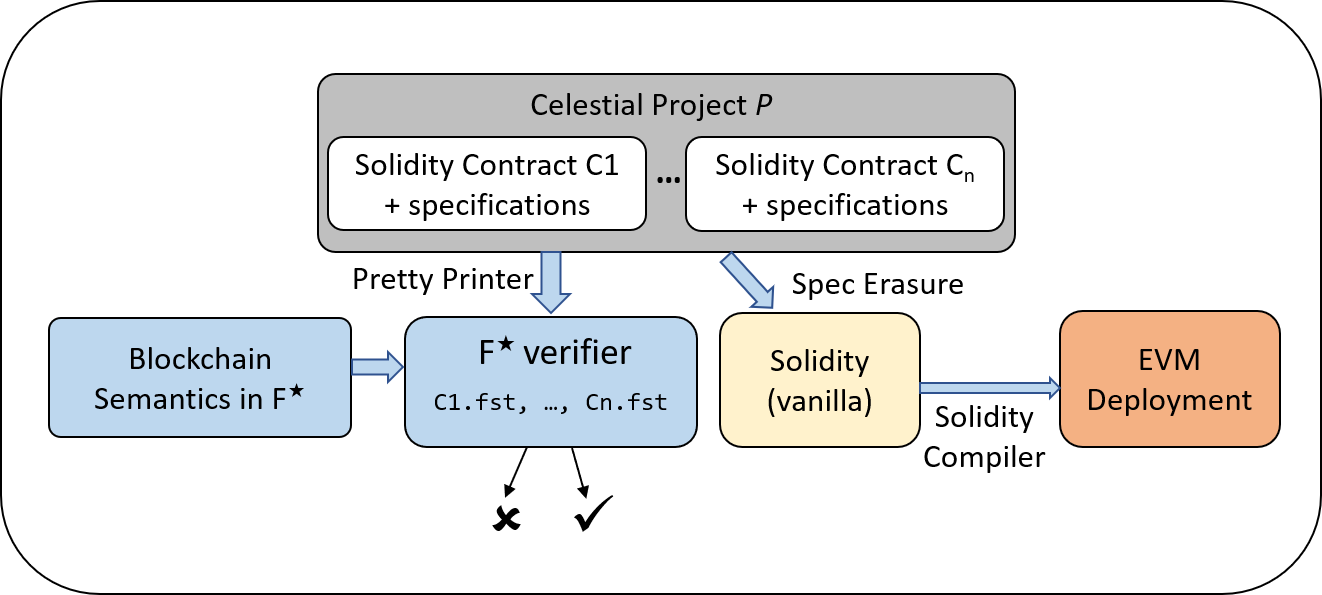
\includegraphics[width=13cm]{logos/CelestialArchitecture.png}
    \caption{Celestial Architecture}
    \label{fig:celestial_architecture}
\end{figure}

This subsection is adddressed to introduce Celestial, 
an analysis tool for Solidity Ethereum-based smart contracs developed by the reasearch team of Microsoft India.
\autoref{fig:celestial_architecture} shows the its architecture. 

The developes provide functional requirements for formally veryfing their specifications. The input file is labeld 
It gives programmers the ability to create functional requirements for their contracts. 
The input file is labelled as ".cel", it is the solidity file, with the added specification expressed in notes. 
When the grammar is checked, the contract and the specifications are translated in F* for having the verified verdict. 

\autoref*{lst:CelestialCode} shows an example of input file. The invariants are expressed in a sort of functions. 
At the beginning of a function, the specification can be expressed, regarding precondition, postcondition and so on. 
One of these can involve the keyword modifies, which specifies the variable that can be modified in the function, or tx\_reverts, 
which states the possible condition that a function can revert. 
The Solidity implementation of the function is kept.
\begin{lstlisting} [language=Solidity, caption={Celestial example specifications}, label={lst:CelestialCode}]
    contract SimpleMarketplace {
        // contract fields
        invariant balanceAndSellerCredits {
            balance >= totalCredits &&
            totalCredits == sum_mapping ( sellerCredits )
        }
        //function 
        function buy ( address itemId ) public
            modifies [ sellerCredits , totalCredits , itemsToSell ,
            log ]
            tx_reverts !( itemId in itemsToSell ) || value != itemsToSell [ itemId ].price
            || value + totalCredits > uint_max
            post (!( itemId in itemsToSell ) && sellerCredits [ seller ] == old ( sellerCredits ) [seller = > sellerCredits [ seller ] + value ]
            && log == ( eItemSold , sender , itemId ) :: old ( log ) )
         { // implementation of the buy function }
    }
\end{lstlisting}

F* is a fully dependent type system proof helper and programs verification. 
The authors gave the same reasons for involving F* for the formal proof in a blockchain context.
First, it offers SMT-based automation, which is sufficient for the completely automated verification of real-world smart contracts. 
Second, F* enables the developers to work in a customised state and exception effect mimicking the blockchain semantics since it supports user-defined effects. 
Finally, even though we only use its first-order subset with quantifiers and arithmetic, F* permits expressive higher-order specifications.

Celestial process involves 2 steps: the translation of the specification and the verification of F* start. 
The first one involves a python script, on the other hand the second one entails the intrallation of F* engine. 
The output covers the response of the verification and a generated solidity file, which represents the smart contract without the specifications notes. 

\paragraph{Limitations} 
The authors explained their tool implementation focused on the Solidity constructs used in their case studies, therefore it does not cover some Solidity cases. 

Delegatecall, embedded assembly
It does not take into account syntactic elements like inheritance, abstract contracts, tuple types, delegatecall and  embedded assembly

Most of these only offer syntactic sugar, which CELESTIAL's future iterations should find simple to support.
Arrays and structs cannot presently be passed as parameters to functions in our implementation. 

Loops are allowed in the smart contracts, however the tool does not suppert loops invariants.
When external contracts are called, reentrant behaviour can result, in which the external contract contacts the caller back.
Reasoning about reentrant actions is frequently counterintuitive.
Celestial forbids these actions, this property is called "external callback freedom" (ECF). It states that every callback execution 
in a contract is equivalent to some activity without reentrancy.
So Celestial assumes that there is no callback during the external call.
Programmers can use the tool to create and support the specifications of their own contracts without making any assumptions about the behaviour of external contracts. 

\subsection{Echidna}
\label{sec:Specification:Echidna}
Echidna is an open-source smart contract fuzzer, developed by \citet{Echidna}, which makes it easy to automatically generate tests to detect violations in
assertions and custom properties.
Rather than relying on a fixed set of pre-defined bug oracles to detect vulnerabilities
during fuzzing campaigns, Echidna supports three types of proper-
ties: 
\begin{itemize}
    \item user-defined properties (for property-based testing);
    \item assertion checking;
    \item gas use estimation.
\end{itemize}

Figure \autoref{fig:echdina_architecture} depicts the Echidna architecture as a two-step process: pre-processing and fuzzing.
The tool starts with a collection of contracts that have been supplied, as well as attributes that have been integrated into one of the contracts.
Echidna uses Slither , smart contract static analysis framework presenet in \autoref{sec:WithoutSpecification:Slither}, to build and analyse the contracts in order to find relevant constants and functions that directly handle Ether (ETH).
The fuzzing effort begins in the second stage. 
Using the application binary interface (ABI) given by the contract, significant constants stated in the contract, 
and any previously gathered sets of transactions from the corpus, this iterative procedure creates random transactions. 
When a property violation is detected, a counterexample is created to indicate the smallest and most basic sequence of operations that caused the failure. 

\begin{figure}
    \centering
    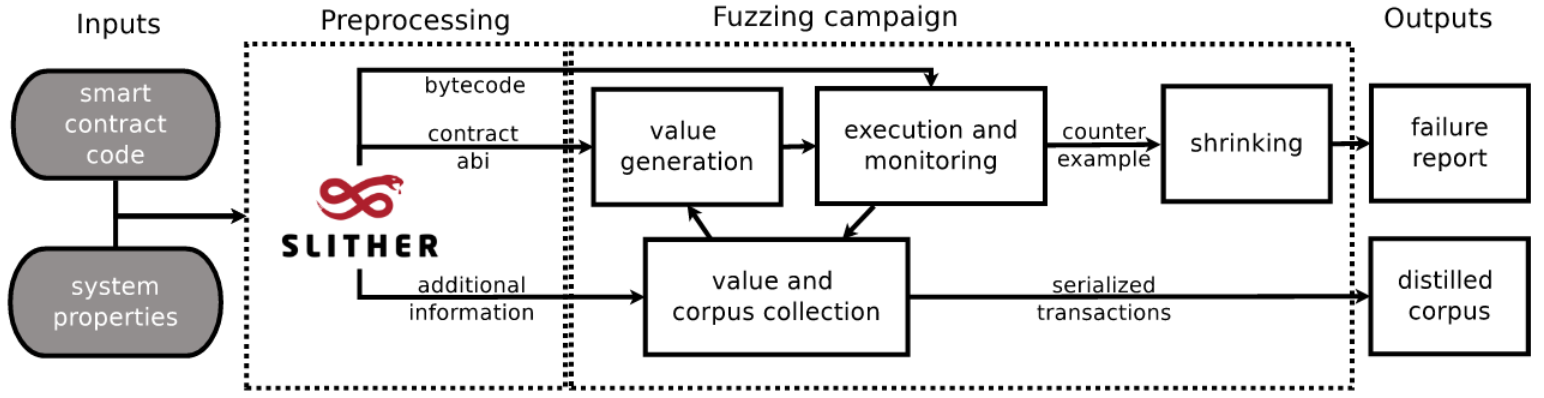
\includegraphics[width=10cm]{logos/echidna.png}
    \caption{Echidna architecture}
    \label{fig:echdina_architecture}
\end{figure}

The code \autoref{lst:EchidnaCode} provides an example of invariant in Echdina context. The Solidity contract contains a vulnerability a the backdoor function. The output of the terminal is presented in Listing \autoref{lst:EchidnaResult}: the attacker. For breaking the property, can call in order the tunctions airdrops() and backdoor()

\begin{lstlisting} [language=Solidity, caption={Solidity smart contract implementing a vulnerable Token and an Echidna invariant function.}, label={lst:EchidnaCode}]
contract Token{
    mapping(address => uint) public balances;
    function airdrop() public{
        balances[msg.sender] = 1000;
    }
    function consume() public{
        require(balances[msg.sender]>0);
        balances[msg.sender] -= 1;
    }
    function backdoor() public{
        balances[msg.sender] += 1;
    }
    function echidna_balance_under_1000() public view returns(bool){
        return balances[msg.sender] <= 1000;
    }
}
\end{lstlisting}

The tool can be even used to test assertions. 
The aim is equivalent of the invariant testing methodology, 
but in this case properties are expressed using the Solidity annotation of assertion.

\begin{lstlisting} [caption={Tool's result after the execution of the precious code.}, label={lst:EchidnaResult}]
    $ echidna-test testtoken.sol --contract TestToken
    ...
    echidna_balance_under_1000: failed!
    Call sequence, shrinking (1205/5000):
    airdrop()
    backdoor()

    ...
\end{lstlisting}


\subsection{Solc-Verify}
\label{sec:Specification:Solc-Verify}

\citet{SolcVerify} present solc-verify, a source-level verification tool for
Ethereum smart contracts. It takes smart contracts written
in Solidity and discharges verification conditions using modular program
analysis. It is built on top of the Solidity compiler, so it reasons at the level of the contract source code. 
Becuase of that, Solc-verify is able to reason about high-level contract attributes 
while accurately modeling low-level language semantics.

Solc-verify is implemented as an extension to the Solidity compiler.
It accepts a collection of Solidity contracts, including specification annotations, and uses 
the Boogie verifier and SMT solvers to discharge verification conditions. 

As \citet{SolcVerify_2} explain, Solc-verify translates the annotated contracts to the Boogie Intermediate Verification
Language (IVL). The key idea of the translation is to encode state variables as global heaps
and functions as procedures. Solc-verify relies on the Boogie verifier to perform modular
verification by discharging verification conditions to SMT solvers. The verification conditions
encode the function body while assuming the preconditions, and then check if postconditions
hold. In this process, function calls are replaced by their specification and loops by their
invariants (modularity). Finally, the results are back-annotated to the Solidity source.

\autoref{lst:SimpleBank} present an example of annotation, which states that the contract will ensure
that the sum of individual balances is equal to the total balance in the bank.


\begin{lstlisting} [language=Solidity, caption={An example Solidity smart contract implementing a simple bank with SolcVerify annotations.}, label={lst:SimpleBank}]
pragma solidity >=0.7.0;

/**
 * @notice invariant __verifier_sum_uint(balances) <= address(this).balance
 */
contract SimpleBank {
    mapping(address=>uint) balances;

    function deposit() public payable {
        balances[msg.sender] += msg.value;
    }

    function withdraw(uint256 amount) public {
        require(balances[msg.sender] > amount);
        bool ok;
        (ok, ) = msg.sender.call{value: amount}(""); // Reentrancy attack
        if (!ok) revert();
        balances[msg.sender] -= amount;
    }
}
\end{lstlisting}

\citet{SolcVerify_3} on GitHub repository, present the specification annotations. Those must be included in special documentation comments (/// or /** */) and must start with the special doctag @notice. 
They must be side-effect free Solidity expressions (with some verifier specific extensions) and can refer to variables within the scope of the annotated element. Functions cannot be called in the annotations, except for getters.
The currently available annotations are listed below. 

\begin{itemize}
    \item Function pre/postconditions can be attached to functions. Preconditions are assumed before executing the function and postconditions are checked (asserted) in the end. The expression can refer to variables in the scope of the function. The postcondition can also refer to the return value if it is named.
    \item Contract level invariants can be attached to contracts. They are included as both a pre- and a postcondition for each public function. The expression can refer to state variables in the contract (and its balance).
    \item Loop invariants can be attached to for and while loops. The expression can refer to variables in scope of the loop, including the loop counter.
    \item Modification specifiers can be attached to functions. The target can be a (1) state variable, including index and member accesses or (2) a balance of an address in scope. Note however, that balance changes due to gas cost or miner rewards are currently not modeled.
    \item Event data specification can be attached to events that should be emitted when certain data changes. 
    Events can declare the state variable(s) they track for changes, or in other words, the variables for which the event should be emitted on a change.
\end{itemize}

\section{Tools without specification}
\label{sec:Tools:WithoutSpecification}

\subsection{SmartTest}
\label{sec:WithoutSpecification:SmartTest}

SmartTest is a safety analayzer for Ethereum smart contracts develeoped by \citet{SmarTest}. 
It adopts a symbolic execution technique for effectively detecting vulnerable transaction sequences. 
The main challenge of the project involves the tool to find transaction sequences,
revealing the vulnerabilities of the analysed smart contract. Therefore, bugs are discoved as the cause of the interaction of multiple transactions.
The purpose of SmartTest is to automatically deliver vulnerable transaction sequences, 
which demostrate the weaknesses of the smart contract.
The main idea is to build a statistical model using known vulnerable transaction sequences and use it to direct symbolic execution toward 
more successfully detecting unknown vulnerabilities. 
Symbolic execution is guided by statistical language models, so it can prioritize transacion sequences which are likely to reveal vulenrablities.
This statregy involves firstly to run unguided symbolic
execution on existing vulnerable contracts, then to learn a probablity distribution over vulnerable transaction sequences.

The tool is implemented as an extension of VeriSmart \autoref{sec:WithoutSpecification:VeriSmart}.
SmartTest is build on top of that, adding its own functionalities:
\begin{itemize}
    \item symbolic execution with a language model.
    \item Symbolic executor for transaction sequences.
    \item Constraint solving optimization.
\end{itemize}
The installation of VeriSmart is necessary for running the tool. After that, the command \autoref{lst:SmarTestRun} is run for using VeriSmart in SmarTest mode.
\begin{lstlisting} [caption={SmarTest Command.}, label={lst:SmarTestRun}]
    ./main.native -input examples/leak_unsafe.sol -mode exploit -exploit_timeout 10
\end{lstlisting}

The report \autoref{lst:SmarTestReport} shows an example of output of SmarTest, which provides the sequence of funtions for exploiting the found bug.
\begin{lstlisting} [caption={SmarTest Example Report.}, label={lst:SmarTestReport}]
    [5] [IO] line 39, (balance[_to] + _value) : disproven, 14.528264s
    1: Example
       {}
       {msg.sender: #x0000000000000000000000000000000000010000,
        msg.value: 0}
    2: approve
       {_spender: #x0000200000000000000000000000000000000000,
        _value: 44365792925664701906080996193724747326645573793336555789802397725137091694592}
       {msg.sender: #x0000000000000000001000000000000000000000,
        msg.value: 0}
    3: mintToken
       {_target: #x0000000000000000001000000000000000000000,
        _amount: 87371285831589357636669861644764241805818792173739087408632338890371299803136}
       {msg.sender: #x0000000000000000000000000000000000010000,
        msg.value: 0}
    4: transferFrom
       {_from: #x0000000000000000001000000000000000000000,
        _to: #x0000000000000000001000000000000000000000,
        _value: 44365787749354941813158155617657849918564739183862151684054205258595743830016}
       {msg.sender: #x0000200000000000000000000000000000000000,
        msg.value: 0}

\end{lstlisting}

The detection of  the following six types of security-critical vulnerabilities are supported by the tool: integer over/underflow, 
assertion violation, division-by-zero, 
ERC20 standard violation, Ether-leaking vulnerability (e.g., 
unauthorized access to transfer), and suicidal vulnerability 
(e.g., unauthorized access to selfdestruct).
In the paper, the authors  focus on just those, without considering vulnerabilities that require analysis of
the interaction of multiple contracts to demonstrate the flaws 
(e.g., reentrancy).





\subsection{Slither}
\label{sec:WithoutSpecification:Slither}
Slither is described by \citet{Slither} as an open-source static analysis framework.
It uses its own intermediate representation, SlithIR, which was created to simplify static analysis of Solidity code. 
Concolic analysis, taint analysis, and control flow checking are involved for detecting a variety
of security vulnerabilities. It is designed to provide
granular information about smart contract code and the flexibility necessary to support many applications.

It is mainly used for:
\begin{itemize}
    \item Automated vulnerability detection: a large variety of
    smart contract bugs can be detected without user inter-
    vention.
    \item Automated optimization detection: Slither detects code
    optimizations that the compiler misses.
    \item Code understanding: printers summarize and display
    contracts' information to aid in the study of the codebase.
    \item Assisted code review: through its API, a user can interact
    with Slither.
\end{itemize}

Slither implements more than twenty bug detectors, regarding reetrancy, Uninitialized variables,
Shadowing and many other. The tool allows the developers to integrate more detectors, therefore it extends Slither's capabilities
to detect more advanced bugs.

\citet{SlitherGitHub} is written in python 3 and it is published on GitHub.
During the installation, I did not find any particular issues.

\subsection{Mythril}
\label{sec:WithoutSpecification:Mythril}
Mythril is a security analysis tool for Ethereum smart contracts. It was introduced by \citet{Mythril}.

The tool  relies on concolic analysis, taint analysis and control flow checking of the EVM bytecode to
prune the search space and to look for values that allow exploiting
vulnerabilities in the smart contract.
It is targeted at finding common vulnerabilities, 
and is not able to discover issues in the business logic of an application. \citet{SWCRegistry}'s taxonomy of vulnerabilities is used by Mythril for classify them. 
Listig \autoref{lst:MythrilOutput} illustrates an example of output of Mythril analysis. 
At the secocond line, there is the reference to the vulnerability classified by SWC Registry with the ID of 110 (Assert Violation).


\begin{lstlisting} [caption={Example of the output of Mythril Analysis.}, label={lst:MythrilOutput}]
==== Exception State ====
SWC ID: 110
Severity: Medium
Contract: Token
Function name: transferArray(address[],uint256[])
PC address: 4385
Estimated Gas Usage: 944 - 6585
An assertion violation was triggered.
It is possible to trigger an assertion violation. Note that Solidity assert() statements should only be used to check invariants. Review the transaction trace generated for this issue and either make sure your program logic is correct, or use require() instead of assert() if your goal is to constrain user inputs or enforce preconditions. Remember to validate inputs from both callers (for instance, via passed arguments) and callees (for instance, via return values).
--------------------
In file: test.sol:309

function transferArray(address[] tos, uint256[] values) public returns (bool) {
        for (uint8 i = 0; i < tos.length; i++) {
            require(transfer(tos[i], values[i]));
        }

        return true;
    }

--------------------

\end{lstlisting}

\subsection{Oyente}
\label{sec:WithoutSpecification:Oyente}

\subsection{Maian}
\label{sec:WithoutSpecification:Maian}

\chapter{Outcome for individual tools}
\label{ch:Running}
Fomal specifications, outcomes, time of running, no comparison, single description, outliers (performe very well or very baddly), 
difficulties in the installation and running 


Detalais regarding what I did for running the test, so for each tool I describe the setting for each scripts.


\subsection{SolcVerify}
Notes:
\begin{itemize}
    \item inheritance allowed 
    \item it worked well with the codes (Solidity Version 7)
    \item the analysed files are still in solidity 
    \item grammar language very intuitive 
    \item it allwos even not flat contract 
\end{itemize}
It works better than Celestial 

\subsection{Celestial}
Notes:
\begin{itemize}
    \item no inheritance
    \item no struct and no array as parameter in function 
    \item total different language 
    \item more grammar for the language 
    \item A lot of grammar 
    \item no address(this), it gives error in fstar
    \item problem with internal functions , fstar could not find the identifier (BZX) 
    \item not so clear which property is violeted  
    \item no loop, neither invariant neither written
\end{itemize}

Uranium: false positive

Spartan: it works good 

bZX: about properties it worked properly, problem with internal functions 

BurgerSwap \& DirtyDogs \& SurgeProcol: no reentrancty bc Calling external contracts are avoided.
Contract Local Reasoning: Calling external contracts
can lead to reentrant behavior where the external contract
calls back into the caller, which is often difficult to reason
about. CELESTIAL disallows such behaviors by checking for
external callback freedom (ECF) [28], [42] which states that
every contract execution that contains a reentrant callback is
equivalent to some behavior with no reentrancy. When this
property holds, it is sufficient to reason about non-reentrant

Aku: it didn't work with the loop so rewrite the contract, but it worked 

Cover Protocol: celestial doesn't recognize memory and storage keyword

\subsection {Manticore}

BurgerSwap \& DirtyDogs \& SurgeProcol: no reentrancy, bc it gives always a fake positive
You can test the Reentrancy just with the tool without specification, runninng Manticore as Scanner 

Spartan: worked well
Uranium: fake positive

Aku: Worked well , it sayes that the rule about claimProject is broken just if everybid is 1 

\subsection {Echidna}
Spartan: it worked correctly and it gave even the transaction oreder, tested with assertions and with test Function

Aku: worked well , it found the correct sequence of transaction for block the contract 

Uranium: it worked prorly, it gave the list of actions to do 

Cover Protocol: worked good


BZX: verified with the assertion but it woked proeprly



\subsection{Manticore}

\subsection{Certora}

\subsection{Tool without Specifiction}
Name of the framwork for running the tools : \href{https://smartbugs.github.io/}{smartbugs}

The framework implements a container which contains the correct enviroment for running the tools: 

\begin{itemize}
    \item HoneyBadger
    \item Maian
    \item Manticore
    \item Mythril
    \item Osiris
    \item Oyente
    \item Securify
    \item Slither
    \item Smartcheck
    \item Solhint
    \item Conkas
\end{itemize}

Withing these I would choose Maian, Manitcore Scanner, Mythril, Osiris, Oyent, Slither.

We run SmartTest which is not implemented in the container.

So in total 6 tools, bc Manticore is already counted.

In total we have 11 tools more or less.


